\documentclass[thesis.tex]{subfiles}
\begin{document}
\chapter{Introduction}
\label{sec:introduction}

\section{Overview}

In the modern era, anyone can go online, search for any topic in which they are interested, and immediately find hundreds, if not thousands, of documents related to that topic. The current power of technology gives people the possibility to learn about almost anything, at least in theory. In reality however, it is often the case that documents are written in a relatively complex way, and/or require prior knowledge in a particular field before truly understanding the material. This is especially problematic for children, but also is an issue for adults with learning disabilities, foreign language learners, or other adults simply trying to learn about a completely new field. To solve this problem, we can consider the task of text simplification.

Automated text simplification is the process that involves transforming a complex text into one with the same meaning that can be more easily read and understood by a broader audience \citep{saggion2017automatic}. This process can include several sub-tasks such as lexical and phrasal simplification \citep{devlin1998use,shardlow2013cw}, reordering \citep{chandrasekar1997automatic,feblowitz2013sentence}, deletion, and sentence splitting \citep{zhu2010monolingual}. 

\begin{figure}[H]
    \centering
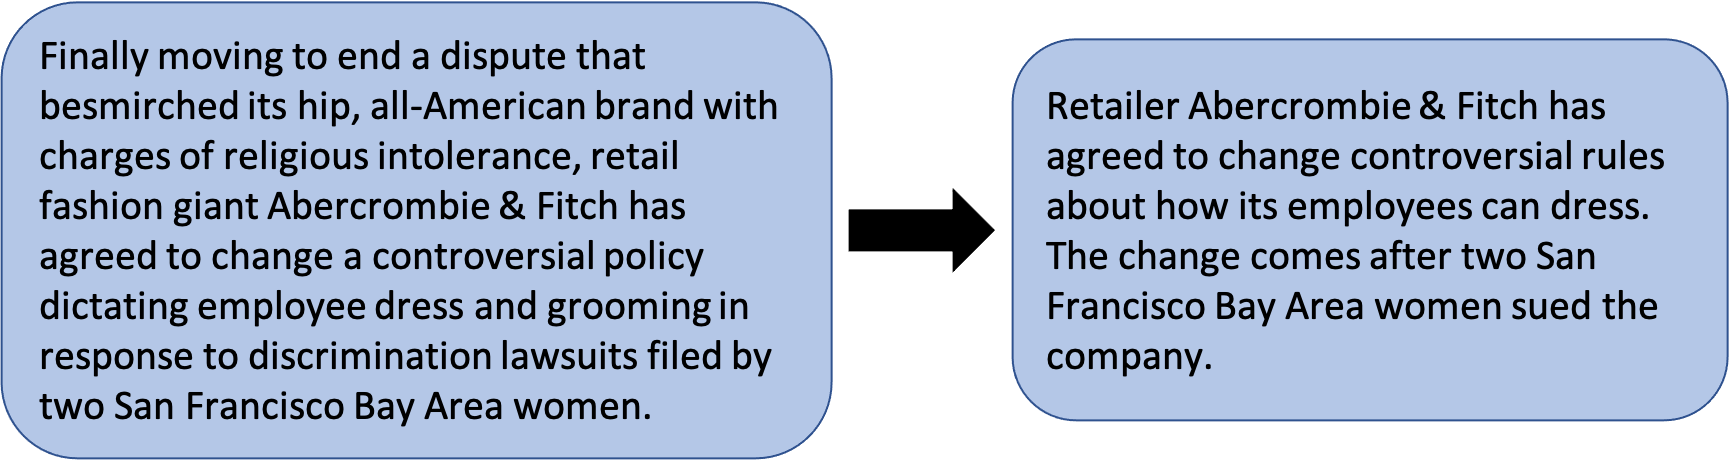
\includegraphics[width=\linewidth]{pictures/intro_example.png}
\caption{An example of an ideal output from a text simplification system. On the left, we show a long and complex text. On the right, we show a simplified version of this text, which preserves the meaning of the original text.}
\label{fig:intro_example}
\end{figure}

As a grounding example that shows these sub-tasks in practice, let's consider the complex text shown on the left of Figure \ref{fig:intro_example} and its simplified version written by professional editors from Newsela\footnote{Newsela is a commonly used simplification corpus introduced by \cite{xu2015problems}, discussed more in Section \ref{sec:newsela}.}, shown on the right. As examples of phrasal simplification, we see that \textit{policy} was changed to \textit{rules}, and \textit{in response to} was changed to \textit{after}. As a more syntactic modification, the final part of the complex text, \textit{discrimination lawsuits filed by two San Francisco Bay area women}, was re-arranged to be presented in the active voice, \textit{two San Francisco Bay area women sued the company}. The beginning of the complex text, \textit{Finally moving to end a dispute that besmirched its hip, all-American brand with charges of religious intolerance}, has been removed, as this part does not contribute much to the meaning of the original text. Finally, we can see that the main part of the complex text has been split into two sentences; this required the addition of a clause, \textit{The change comes}, in order to preserve grammaticality in the simplified version.

Many recent approaches attempt to formulate text simplification as a monolingual generation task and apply sequence-to-sequence (Seq2Seq) models \citep{nisioi2017exploring,zhang2017sentence,zhao2018integrating}. These have been shown to give state-of-the-art results in machine translation \citep{sutskever2014sequence}, dialogue systems \citep{vinyals2015neural}, and many other natural language processing fields. While these methods have shown improvement over previous statistical and phrase-based approaches, their practical uses are still somewhat limited. There are several reasons for this. First, although recent simplification models generate grammatical output, they do not make all necessary changes to the original text \citep{zhang2017sentence}. Second, there is a lack of quality simplification data available for training \citep{xu2015problems}. Finally, current evaluation metrics have low or negative correlations with human judgments of simplification quality \citep{xu2016optimizing,sulem2018bleu}. Beyond these issues, a higher-level problem is that these models view simplification as translating from a specific complex to a specific simple level. However, texts can be written at many complexity levels, and even the same text can be of varying difficulty depending on a reader's background knowledge. Moreover, a text might contain domain-specific terminology which requires a more detailed explanation to be understood, rather than merely substituting it with a simpler term.
%there are many phrases in a text, such as ``logistic regression", that cannot be more easily understood just by replacing with simpler language; instead, these concepts require a more detailed explanation.

\section{Thesis Statement}

In this thesis, we claim that the textual complexity at any level is not a static value, but instead is influenced both by the surrounding text and especially the knowledge of a particular reader. Thus, in order to create a practically useful simplification system, it is critical to be able to adjust the outputs of our models depending on the situation. 

In the chapters that follow, we demonstrate how this framing can inform and improve simplification systems at three levels: at the word level, where we show how to identify complex words and replace them with simpler substitutes while better taking the surrounding context into account; at the sentence level, where we show how to produce simpler outputs by generating a large number of diverse candidate sequences; and at the document level, where we consider how to identify concepts that are critical to understanding a document, and then how to retrieve related documents from a variety of complexity levels.

%I propose to address the task of creating a practically useful simplification system. Specifically, I plan to show how we can further improve current lexical and sentence-level text simplification systems, while going into more detail about how to most effectively generate diverse candidates. I also propose a potential retrieval-based reformulation of the simplification problem to focus more directly on a key question: how can we help a user more easily learn about specific topics? 

\section{Outline of this Document}

The rest of this document is organized as follows.

\subsubsection{Chapter 2}

We begin with an overview of related work in the field of text simplification, and include a general discussion of generation and language modeling. First, we present previous work specifically focusing on the lexical simplification task, which includes two sub-tasks: identifying complex words in a text (known as complex word identification or CWI), and replacing them with simpler substitutes. We also present several widely-used paraphrase datasets, which can be effectively leveraged for lexical simplification. Next, we briefly discuss corpora used for training sentence simplification systems. We then review several state-of-the-art approaches for training a holistic statistical simplification system, where the input is a complex English sentence and the output is a simple English sentence. The chapter continues with a discussion of Sequence-to-Sequence models, their applications to text simplification, and how to effectively generate outputs at inference time. Subsequently, we discuss in detail several commonly-used metrics for evaluating these systems; in this section, we also discuss the limitations of these metrics, and why human evaluation is still considered the most trustworthy method of evaluation simplification systems. We conclude this section with a discussion of large-scale pre-trained language models.

\subsubsection{Chapter 3}

In Chapter 3, we present our proposed approach to the task of lexical simplification.
%address the task of lexical simplification, which involves replacing difficult words in a text with words that are easier to understand. 
We propose to solve this task in two steps: we first identifying words that are difficult to understand within a text, and then replace them with simpler alternatives that make sense in the same context.

\begin{figure}[H]
    \centering

\includegraphics[width=0.8\linewidth]{pictures/lex_example.png}
\caption{An example sentence with complex words identified by our classifier, and substitutes proposed by our embedding-based lexical simplification model.}
\label{fig:lex_example}
\end{figure}

Specifically, in order to identify complex words, we train a Support Vector Machine (SVM) classifier which uses both word-based and context-based features. To train this classifier, we create a corpus of \textit{in-context} complex and simple words annotated by Amazon Mechanical Turk workers. For the substitution step, we extract candidate substitutes from a large-scale database of simplifying paraphrase rules \citep{pavlick2016simple}. We select the substitutes that best fit each context using a word embedding-based lexical substitution model. We show that our CWI classifier and lexical simplification model yield results that outperform several baseline approaches, and provide a detailed error analysis to show when our methods fall short. This chapter expands on our NAACL 2018 long paper on lexical simplification \citep{kriz2018simplification}.

\subsubsection{Chapter 4}

A simplification model that is useful in practice should not only make lexical or phrasal substitutions, but also perform other operations, such as reordering and deletion. In Chapter 4, we consider the task of sentence simplification, which aims to holistically simplify entire sentences. In this task, we start with a complex English sentence and attempt to generate a simple English sentence that is fluent (i.e. grammatical), adequate (i.e. meaning-preserving), and simpler than the original. In this part of our work, we leverage a Sequence-to-Sequence (Seq2Seq) model, which learns how to perform all simplification operations simultaneously.

Vanilla Sequence-to-Sequence (Seq2Seq) models \citep{sutskever2014sequence} have been shown to work well on this task \citep{nisioi2017exploring}, although they often make very few changes to the original complex sentence \citep{zhang2017sentence}. We address this problem by proposing extensions to the generic Seq2Seq framework at training, inference, and post-inference time. During training, we propose a custom loss function that rewards the model more for correctly generating simpler content words. We do so by multiplying the standard cross entropy loss function by the predicted complexities of each word in our vocabulary. At inference time, rather than using the standard greedy search to generate a single system output, we implement a diverse beam search approach which penalizes candidates that come from the same partial parent output, thus allowing us to explore more of the search space. Finally, at post-inference time we re-rank the multiple generated candidates using external methods to judge the fluency, adequacy, and simplicity of each output. An example output of our model compared with that generated from a vanilla Seq2Seq model is shown in Figure \ref{fig:sentence-example}. While these extensions do result in simpler output sentences, there is a trade-off where we sometimes lose critical information from the original. We again provide an error analysis to discuss limitations of our approach in more detail. This section discusses work from our NAACL 2019 long paper on sentence simplification \citep{kriz2019complexity}.

\begin{figure}[H]
    \centering
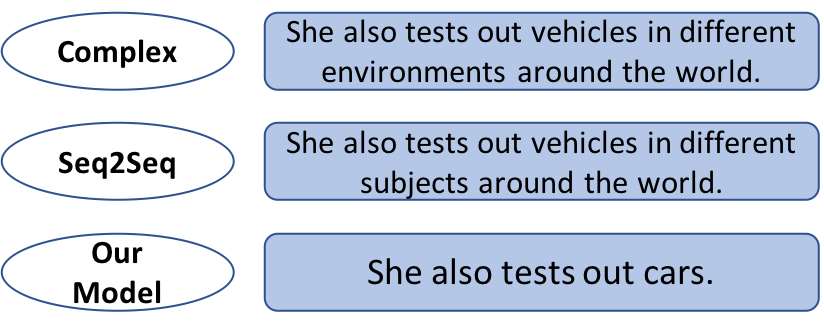
\includegraphics[width=0.5\linewidth]{pictures/sentence-example.png}
\caption{Comparison of a simplification generated by a vanilla Seq2Seq model vs. our proposed model.}
\label{fig:sentence-example}
\end{figure}

We observed that while our sentence simplification method yielded higher performance than previous methods, as measured using standard automatic simplification metrics, the results were more mixed after collecting manual human annotations. Thus, in the last part of this chapter, we discuss the creation of an automatic quality estimation metric that correlates better with human judgments, without requiring a reference sentence for comparison. Given a complex sentence and the corresponding simplified output, we fine-tune BERT \citep{devlin2019bert} to predict its fluency, adequacy, and relative complexity simultaneously. We show that training a single model rather than three separate models results in better performance, likely due to the fact that each individual dimension is somewhat correlated with the others. This section discusses work from our ArXiv short paper on simplification evaluation \citep{kriz2020simple}.

\subsubsection{Chapter 5}

In Chapter 4, we implemented several extensions to Seq2Seq models for the task of text simplification; from these extensions, encouraging diversity at inference time led to significant improvements. This notion of diversity is not unique to text simplification, in fact many NLP generation tasks, including conversational dialogue systems (i.e. chatbots), image captioning, and story generation, can benefit from leveraging diverse candidate outputs for a single input. In Chapter 5, we take closer look at the idea of diversity, and perform an exhaustive comparison of current diverse decoding techniques. In this chapter, we define diversity as the ability of a generative method to create a set of possible outputs that are all valid for a given input, but vary as much as possible in terms of word choice, topic, and meaning.

Early neural machine translation work found that beam search is an effective heuristic to sample likely sequences from conditional language models \citep{sutskever2014sequence}. However, this was initially restricted to tasks where only the most likely output sequence was considered; if we want to use beam search to generate multiple candidates, it has been shown that these tend to only differ in punctuation and/or minor morphological variations \citep{li2016mutual}. A variety of alternatives and extensions to beam search have thus been proposed for generating diverse candidate responses \citep{li2016diversity,vijayakumar2016diverse,kulikov2018importance,tam2019clustered}. Many of these approaches show marked improvement in diversity over standard beam search across a variety of generative tasks. However, there has been little comparison and evaluation of these strategies against each other on a single task. In this work we systematically compare existing diverse decoding methods on two tasks: chatbots and image captioning. We also propose the use of over-sampling followed by re-ranking at post-inference time. 

\begin{figure}[bt]
    \scriptsize
    \begin{subfigure}[l]{0.6\linewidth}
    
\includegraphics[width=\linewidth]{pictures/COCO_val2014_000000155401.jpg}
    \end{subfigure}
    \begin{subfigure}[l]{0.5\linewidth}
    \begin{tabular}{l}
\textbf{Beam Search}  \\
A bus is stopped at a bus stop. \\
A bus is parked at a bus stop. \\
A bus stopped at a bus stop in a city. \\
A bus stopped at a bus stop at a bus stop. \\
A bus that is parked in front of a building. \\ \hline
\textbf{Random Sampling}  \\
A bus parked at a bus stop at a bus stop.  \\
There is a bus that is at the station. \\
A man standing by a bus in a city.  \\
A bus pulling away from the train station. \\
A bus stopped at a stop on the sunny day. \\
    \end{tabular}
    \end{subfigure}
    \caption{An image with the top five captions produced by standard beam search and by random sampling. Note that the latter set is more diverse but of lower quality.}
    \label{first_example}
\end{figure}

In our experiments, we show that if the underlying model performs relatively well on a task, leveraging the increased diversity in a random sampling-based approach will likely lead to high-quality and diverse outputs. On the other hand, if the underlying model performs relatively poorly on the initial task, encouraging too much diversity will likely come at the cost of output quality. This work is based on work from our ACL 2019 long paper on diversity in conditional language models \citep{ippolito2019comparison}; with this paper, Daphne Ippolito and I were co-first authors, and share equal credit for this work.

\subsubsection{Chapter 6}

%Chapters 3 and 4 proposed new methodologies for lexical- and sentence-level simplification systems; however, despite making improvements over previous approaches in both cases, 

In Chapters 3 and 4 our proposed methodologies for lexical- and sentence-level simplification yield better results than previous approaches; however in our error analyses we identified several fluency and adequacy errors that our models still make quite often. At the sentence level, the errors are particularly pronounced the input sentences are long and complex. %when attempting to simplify very long and complex sentences. 
Fine-tuning pre-trained language generation models \citep{radford2019language,brown2020language} could serve to better address some quality issues at the sentence level. However, these models would still fall short at the document level, as the text they generate still contains many long-term inconsistencies \citep{ippolito2020automatic}. Thus, it is currently difficult to scale generation further in order to simplify entire documents without significant loss in meaning.

Due to these issues, Chapter 6 proposes to reformulate the text simplification task.  Given a document $D$ on some topic, we can 1) identify the concepts that are critical for understanding $D$, 2) retrieve a set of documents $D^{\prime}$ related to each concept from a large general corpus, where $D^{\prime}$ contains documents from a variety of complexity levels, and 3) re-rank $D^{\prime}$ to find documents written at levels that are most appropriate for the user. This is an extremely ambitious reformulation; thus the experiments in this Chapter are meant to serve as steps taken towards this final goal.

In the first section of Chapter 6, we discuss our methodology for identifying the critical concepts in a document $D$. There has been an extensive amount of work on keyphrase extraction, a field related to critical concept identification, so first we discuss the most prominent unsupervised methods that have been proposed to identify keyphrases in a single document. Furthermore, we present several simple Wikipedia-based baselines, which extract a set of domain-specific concepts by leveraging the internal Wikipedia category hierarchy. Finally, we describe recent BERT-based keyphrase extraction approaches, and propose a novel BERT-based approach that first identifies several high-quality seed concepts, before iteratively identifying additional concepts based on their similarity to the seed concepts. In order to evaluate these methods on real data, we create a test set consisting of computer science web articles. From there, we collect annotations for each article, and perform a secondary round of adjudication to ensure agreement. When tested on this evaluation set, BERT-based methods interestingly perform worse than previous unsupervised approaches that do not leverage large-scale pre-trained language models.

In the second section of Chapter 6, we focus on the tasks of retrieving related documents at different complexity levels ranked based on embedding similarity, and their re-ranking according to the desired complexity level. For this task, our methodology relies on a mechanism that combines embedding-based text similarity \citep{reimers2019sentence} with a complexity re-ranking module. We conduct experiments in settings of varying difficulty, involving a diverse number of distractor documents. Initially, we leverage Newsela, a parallel corpus of 1,882 news articles rewritten at 5 complexity levels. Given a Newsela article written at complexity level 4 (L4), we attempt to retrieve the rewritten articles from L0, L1, L2, and L3, using the rest of the articles as distractors. 

\begin{figure}[H]
    \centering
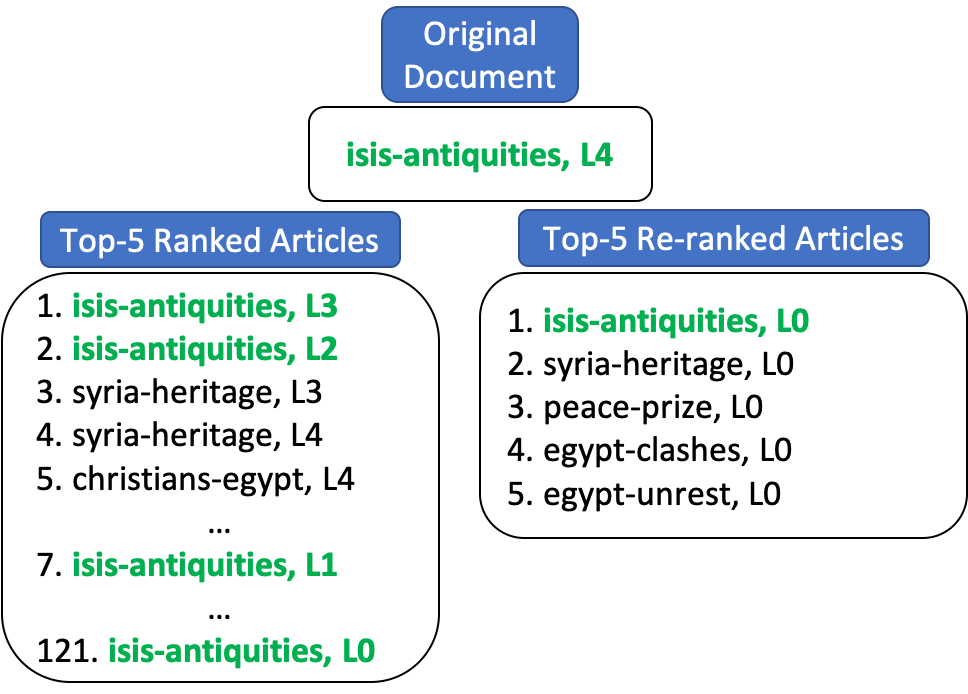
\includegraphics[width=7.5cm]{pictures/retrieval-example.png}
\caption{Given an input article at complexity Level 4 (L4), we show the ranking of aligned articles based on SBERT embedding similarity \cite{reimers2019sentence}, and the output of our re-ranking methodology which boosts articles at the lowest complexity level (L0).}
\label{fig:retrieval-example}
\end{figure}

We show that we can effectively retrieve L3 and L2 documents, as these are the versions with the least amount of changes and, thus, the most similar. However, current embeddings-based retrieval approaches seem to struggle with L1 and especially with L0 documents. To address this, we introduce a re-ranking mechanism which involves fine-tuning BERT to predict document-level complexity \citep{devlin2019bert}. This mechanism allows us to effectively filter out documents at incorrect complexity levels, making our retrieval approach significantly more effective. Finally, in a large-scale experiment, we show that our methodology successfully retrieves related documents at the desired complexity level even in a challenging scenario with over one million candidate documents.

\subsubsection{Chapter 7}

Chapter 7 summarizes the key ideas and take aways from this thesis, along with its limitations and areas for future work.

%With the rise of large-scale pre-trained models, many classification and generation tasks have seen an explosion of improvement \cite{devlin2019bert,radford2019language}. I propose to explore how these models can be leveraged for current simplification-specific tasks. Specifically, I demonstrate that we can fine-tune BERT for predicting the overall quality of sentence simplification systems, as well as sentence- and document-level complexity. In addition, I propose to probe these model architectures to determine if different parts of the network are able to model specific sub-tasks of simplification.

%Finally, after discussing the inherent limitations of current simplification tasks, I will propose our reformulated task, which considers simplification from an information theoretic perspective. If we start with a document $D$ on a given topic, we can break down the problems into three sub-problems. The first is \textit{Concept Identification}, where we identify the concepts within $D$ that are critical to understanding that document; this also can include identifying pre-requisite concepts as well. The second task is \textit{Leveled Document Retrieval}, where for each concept $c$, we need to retrieve a set of documents $D^{\prime}$ related to $c$ from a $variety$ of complexity levels. Finally, the third task is \textit{Document Re-ranking}, where given a set of related documents $D^{\prime}$, we need to select the document that is the most appropriate for the user. We propose initial approaches for each of these tasks, and discuss several of the difficulty that will likely arise.
\biblio
\end{document}
